\documentclass[standalone, version=2.0]{huangfusl-template}
\begin{document}
\begin{tabular}{cc}
    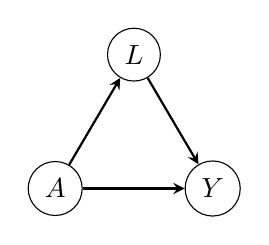
\begin{tikzpicture}
        \node[draw, circle] (A) at (-1, 0) {$A$};
        \node[draw, circle] (Y) at (1, 0) {$Y$};
        \node[draw, circle] (L) at (0, 1.7) {$L$};
    
        \draw[-stealth, thick] (A) -- (L);
        \draw[-stealth, thick] (A) -- (Y);
        \draw[-stealth, thick] (L) -- (Y);
    \end{tikzpicture} &
    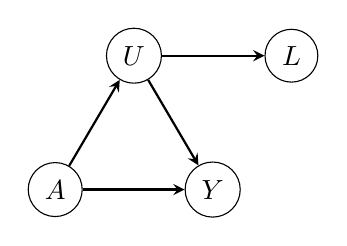
\begin{tikzpicture}
        \node[draw, circle] (A) at (-1, 0) {$A$};
        \node[draw, circle] (Y) at (1, 0) {$Y$};
        \node[draw, circle] (U) at (0, 1.7) {$U$};
        \node[draw, circle] (L) at (2, 1.7) {$L$};
    
        \draw[-stealth, thick] (A) -- (U);
        \draw[-stealth, thick] (A) -- (Y);
        \draw[-stealth, thick] (U) -- (Y);
        \draw[-stealth, thick] (U) -- (L);
    \end{tikzpicture} \\
    proposed graph & true graph
\end{tabular}
\end{document}